\documentclass[11pt,a4paper]{article}

% --- Essential Packages ---
\usepackage[utf8]{inputenc}
\usepackage[margin=1in]{geometry}
\usepackage{amsmath,amssymb,amsfonts}
\usepackage{booktabs}
\usepackage{tabularx}
\usepackage{array}
\usepackage{xcolor}
\usepackage{graphicx}
\usepackage{tikz}
\usetikzlibrary{shapes.geometric, arrows, positioning, calc, fit}
\usepackage{enumitem}
\usepackage{titlesec}
\usepackage{fancyhdr}
\usepackage{listings}
\usepackage{microtype}

% --- Professional Hyperref Configuration (Strictly NO RED BOXES) ---
\usepackage[hidelinks,pdftex,bookmarks=true,bookmarksnumbered=true]{hyperref}
\hypersetup{
    colorlinks=true,
    linkcolor=blue!75!black,
    citecolor=blue!75!black,
    urlcolor=blue!75!black,
    pdfborder={0 0 0}
}

% --- Page Header & Footer Styling (No Top Headers / Rules on any page) ---
\pagestyle{plain}

% --- Section Title Styling ---
\titleformat{\section}{\large\bfseries\color{blue!80!black}}{\thesection}{1em}{}[\titlerule]
\titleformat{\subsection}{\normalsize\bfseries\color{black}}{\thesubsection}{1em}{}
\titleformat{\subsubsection}{\small\bfseries\color{gray!30!black}}{\thesubsubsection}{1em}{}

% --- Code / Register Listings Style ---
\lstset{
    basicstyle=\small\ttfamily,
    breaklines=true,
    backgroundcolor=\color{gray!8},
    frame=single,
    rulecolor=\color{gray!30},
    numbers=none,
    keywordstyle=\color{blue!80!black}\bfseries,
    stringstyle=\color{teal!70!black},
    commentstyle=\color{gray!70!black}\itshape
}

\begin{document}

% ============================================================================
% PAGE 1: TITLE ONLY (STRICTLY ISOLATED AS REQUESTED)
% ============================================================================
\vspace*{\fill}
\begin{center}
    {\LARGE \textbf{Autonomous Robot: Comprehensive Power Management, Subsystem Operating States, and Battery Longevity Analysis}\par}
\end{center}
\vspace*{\fill}
\thispagestyle{empty}
\newpage

% ============================================================================
% SECTION 1: SYSTEM POWER ARCHITECTURE
% ============================================================================
\section{System Architecture \& Dual-Rail Power Distribution}

\subsection{Project Motivation \& Core Objective}
Autonomous mobile robots deployed for mapping, surveillance, and automated inspection are strictly bounded by onboard battery capacity. Running all computational cores, spinning laser scanners, video cameras, and high-power traction motors continuously depletes standard battery packs within an hour. To achieve prolonged operational endurance, this robot implements an intelligent \textbf{multi-tier power management architecture} capable of dynamically transitioning between \textbf{Full Active Cruising Mode} and \textbf{Ultra-Low-Power Deep Sleep Mode}.

By putting idle sensors, drivers, and processor peripherals into coordinated low-power states, the platform achieves a \textbf{27-fold power reduction}, extending standby life from hours to multiple days.

\subsection{Dual-Voltage Rail Distribution Topology}
DC geared motors produce substantial electrical switching noise and inductive voltage spikes (Back-EMF). If logic microcomputers and sensitive sensors share a common unregulated power bus with motors, high-current transient draws cause voltage brownouts, crashing the processor and corrupting inertial measurements.

To solve this, our hardware architecture strictly segregates power into two distinct electrical domains:
\begin{itemize}[noitemsep]
    \item \textbf{High-Power Motor Bus (11.1V Direct Battery Rail):} Connects the 3-Cell Lithium-Polymer (3S LiPo) battery pack directly to the motor driver high-power pins ($V_M$) on two Toshiba TB6612FNG H-bridge ICs. This isolates electrical drive surges from sensitive computation.
    \item \textbf{Regulated Logic Rail (5.0V Buck-Regulated Rail):} Connects the 11.1V battery output to a high-efficiency DC-DC step-down switching regulator (90\% conversion efficiency). This delivers clean, ripple-free 5.0V power to the Raspberry Pi 3 Model B, the RPLiDAR A1 processing engine, the MPU-6050 breakout, and the TB6612FNG digital logic gates ($V_{\text{CC}}$).
    \item \textbf{Secondary Sensor Rail (3.3V Low-Dropout Rail):} Sourced directly from the Raspberry Pi power management IC, providing clean power to the Sony IMX219 CSI camera sensor, the MPU-6050 internal MEMS circuitry, and $I^2$C pull-up resistors.
\end{itemize}

\begin{figure}[htbp]
\centering
\resizebox{\linewidth}{!}{
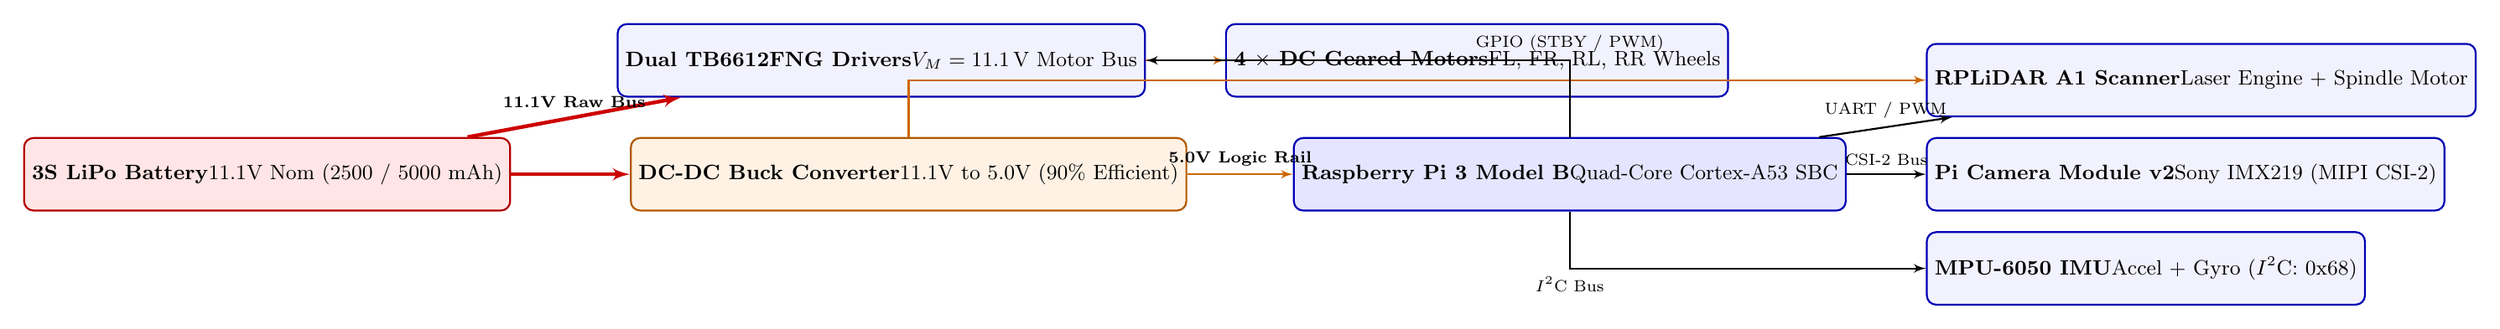
\begin{tikzpicture}[node distance=1.5cm, auto,
    block/.style={rectangle, draw=blue!70!black, fill=blue!5, rounded corners, thick, text centered, minimum width=3.2cm, minimum height=1.1cm, font=\small},
    bus/.style={draw=red!80!black, ultra thick, -latex'},
    pwr/.style={draw=orange!80!black, thick, -latex'},
    sig/.style={draw=black, thick, -latex'}
]
    \node [block, fill=red!10, draw=red!70!black] (bat) {\textbf{3S LiPo Battery}\\11.1V Nom (2500 / 5000 mAh)};
    \node [block, right=1.8cm of bat, fill=orange!10, draw=orange!70!black] (buck) {\textbf{DC-DC Buck Converter}\\11.1V to 5.0V (90\% Efficient)};
    \node [block, above right=0.6cm and 1.6cm of bat] (driver) {\textbf{Dual TB6612FNG Drivers}\\$V_M = 11.1\,\text{V}$ Motor Bus};
    \node [block, right=1.2cm of driver] (motors) {\textbf{4 $\times$ DC Geared Motors}\\FL, FR, RL, RR Wheels};
    
    \node [block, right=1.6cm of buck, fill=blue!10] (pi) {\textbf{Raspberry Pi 3 Model B}\\Quad-Core Cortex-A53 SBC};
    \node [block, above right=0.3cm and 1.2cm of pi] (lidar) {\textbf{RPLiDAR A1 Scanner}\\Laser Engine + Spindle Motor};
    \node [block, right=1.2cm of pi] (cam) {\textbf{Pi Camera Module v2}\\Sony IMX219 (MIPI CSI-2)};
    \node [block, below right=0.3cm and 1.2cm of pi] (imu) {\textbf{MPU-6050 IMU}\\Accel + Gyro ($I^2\text{C: } 0\text{x}68$)};

    % Power Connections
    \path [bus] (bat) -- node[above, font=\scriptsize\bfseries] {11.1V Raw Bus} (driver);
    \path [bus] (bat) -- (buck);
    \path [pwr] (driver) -- (motors);
    \path [pwr] (buck) -- node[above, font=\scriptsize\bfseries] {5.0V Logic Rail} (pi);
    \path [pwr] (buck) |- (lidar);
    \path [sig] (pi) -- node[above, font=\scriptsize] {CSI-2 Bus} (cam);
    \path [sig] (pi) -- node[above, font=\scriptsize] {UART / PWM} (lidar);
    \path [sig] (pi) |- node[below, font=\scriptsize] {$I^2$C Bus} (imu);
    \path [sig] (pi) |- node[above, font=\scriptsize] {GPIO (STBY / PWM)} (driver);
\end{tikzpicture}
}
\caption{System dual-rail power distribution and hardware control topology.}
\label{fig:power_arch}
\end{figure}

\newpage

% ============================================================================
% SECTION 2: SUBSYSTEM OPERATING STATES
% ============================================================================
\section{Subsystem Operating States: Active Mode vs. Deep Sleep Mode}

Every hardware device on the robot possesses distinctive electrical operational modes. Below is the operational detail for each subsystem.

\subsection{Host Computing Processor: Raspberry Pi 3 Model B}
The host Single Board Computer executes the real-time Linux operating system, obstacle detection, path planning, and wireless WebSocket communication.
\begin{itemize}
    \item \textbf{Active Mode:} All four 64-bit ARM Cortex-A53 cores operate at peak frequency (1200 MHz) under dynamic frequency scaling. Wi-Fi telemetry streams continuous telemetry data, USB controllers are fully powered, and hardware PWM pins control motor speed. Active power dissipation is approximately \textbf{3.60 Watts} (720 mA at 5V).
    \item \textbf{Sleep Mode:} CPU cores are throttled down to 600 MHz in low-power governor mode. The HDMI transmitter circuitry is de-energized via software command, status LEDs are turned off, and external USB ports enter suspended state. Power consumption drops by \textbf{80.6\%} down to \textbf{0.70 Watts} (140 mA at 5V) while remaining alert for network or hardware wake triggers.
\end{itemize}

\subsection{Primary Range Scanner: RPLiDAR A1 360$^\circ$ Optical Scanner}
The Slamtec RPLiDAR A1 performs laser triangulation using an infrared laser and optical sensor mounted on a rotating spindle.
\begin{itemize}
    \item \textbf{Active Mode:} The infrared laser diode pulses 8,000 times per second, while the coreless DC spindle motor spins the turret at 330 RPM (5.5 Hz) via a 65\% PWM signal. It captures 360$^\circ$ distance points up to 12 meters for real-time occupancy grid mapping. Power draw is \textbf{1.90 Watts} (380 mA at 5V).
    \item \textbf{Sleep Mode:} The host issues a digital STOP command packet over serial UART. The internal laser diode immediately shuts off, and the motor PWM duty cycle is set to 0\%, halting mechanical rotation. Only a minimal optocoupler receiver stays active, reducing power by \textbf{97.9\%} down to \textbf{0.040 Watts} (8 mA at 5V).
\end{itemize}

\subsection{Inertial Measurement Unit: MPU-6050 6-DOF IMU}
The MPU-6050 combines a 3-axis gyroscope, a 3-axis accelerometer, and an onboard Digital Motion Processor communicating over $I^2$C at 400 kHz.
\begin{itemize}
    \item \textbf{Active Mode:} Gyroscopes and accelerometers sample motion at 100 Hz. The internal processor continuously calculates robot tilt, pitch, and yaw orientation to prevent odometry drift. Active power draw is \textbf{12.5 milliwatts} (3.8 mA at 3.3V).
    \item \textbf{Sleep Mode:} Gyroscope drive circuits and internal clock synthesizers are powered down. The accelerometer enters low-power cycle mode, drawing only microamps. It acts as an active physical sentry: using its built-in Wake-on-Motion interrupt, if any disturbance or collision occurs, it instantly pulses its interrupt line to wake the host computer. Sleep power drops by \textbf{99.8\%} down to \textbf{16.5 microwatts}.
\end{itemize}

\subsection{Vision Subsystem: Raspberry Pi Camera Module v2}
Equipped with an 8-megapixel Sony IMX219 sensor connected directly via 2-lane MIPI CSI-2.
\begin{itemize}
    \item \textbf{Active Mode:} Captures 720p video at 30 frames per second directly into the hardware Image Sensor Pipeline for live human teleoperation and visual obstacle verification. Power draw is \textbf{0.825 Watts} (250 mA at 3.3V).
    \item \textbf{Sleep Mode:} The video device pipeline is closed, and MIPI transceivers enter high-impedance mode. Sensor readout circuitry powers down, slashing power by \textbf{99.4\%} down to \textbf{4.95 milliwatts}.
\end{itemize}

\subsection{Drive Actuation: Dual TB6612FNG Drivers \& 4WD Geared Motors}
Locomotion is delivered by four independent DC geared motors driven by two dual-channel H-bridge ICs.
\begin{itemize}
    \item \textbf{Active Mode:} H-bridges switch at 1 kHz PWM with 60\% duty cycle to cruise smoothly at 0.35 meters per second. The four motors collectively draw 1.68 Amps from the 11.1V battery rail, consuming \textbf{18.65 Watts}. If an obstacle is detected within 50 cm, dynamic short-circuit braking (shorting motor terminals to ground) is engaged, stopping kinetic rotation within 120 ms.
    \item \textbf{Sleep Mode:} The host Raspberry Pi asserts logic LOW on the hardware Standby (STBY) pin of both drivers. This instantly places all output power MOSFETs into high-impedance (Hi-Z) mode and powers down internal charge pumps. Motor current drops to 0 mA and driver idle leakage drops below 1 microamp (\textbf{11 microwatts}), completely eliminating stationary battery drain.
\end{itemize}

\newpage

% ============================================================================
% SECTION 3: STEP-BY-STEP TRANSITION PROTOCOLS
% ============================================================================
\section{Chronological Step-by-Step Transition Procedures}

To prevent inductive Back-EMF voltage spikes, preserve occupancy maps, and ensure deterministic battery savings, the robot executes verified sequential shutdown and start-up protocols.

\subsection{Active-to-Sleep Transition Procedure (Shutdown Sequence)}
The transition from full active cruising to deep sleep completes in approximately \textbf{800 milliseconds} across seven sequential steps:
\begin{enumerate}[noitemsep]
    \item \textbf{Step 1 --- Dynamic Motor Braking (150 ms):} The motion controller decelerates motors to zero speed and applies dynamic short-circuit braking ($IN1=IN2=\text{HIGH}$) for 120 ms to completely eliminate residual vehicle kinetic energy.
    \item \textbf{Step 2 --- Hardware Driver Standby (5 ms):} The host controller pulls the hardware \texttt{STBY} pin to logic LOW on both TB6612FNG modules. Output FETs enter high-impedance state, cutting motor coil currents to zero.
    \item \textbf{Step 3 --- Optical LiDAR Shutdown (200 ms):} The serial STOP command packet is transmitted, immediately depowering the laser emission diode. Spindle motor PWM is set to 0\%, allowing the mechanical turret to coast to a halt.
    \item \textbf{Step 4 --- Camera Pipeline Closure (45 ms):} The MIPI video stream buffer is released, and the Sony IMX219 image sensor enters low-power standby mode.
    \item \textbf{Step 5 --- IMU Sentry Configuration (10 ms):} The MPU-6050 writes register commands disabling gyroscopes and activates the Wake-on-Motion interrupt with a 32 mg movement threshold.
    \item \textbf{Step 6 --- Host OS Downclocking (350 ms):} Active file system caches are flushed to SD storage, the CPU frequency is scaled down to 600 MHz, and HDMI video circuitry and status LEDs are disabled.
    \item \textbf{Step 7 --- System FSM State Finalization (40 ms):} The supervisory software logs the sleep event to flash memory and broadcasts the \texttt{LOW\_POWER\_SLEEP} state update across the network.
\end{enumerate}

\subsection{Sleep-to-Active Wake-Up Procedure (Start-up Sequence)}
When woken by a network packet, timer, or physical motion interrupt, the robot boots in approximately \textbf{650 milliseconds}:
\begin{enumerate}[noitemsep]
    \item \textbf{Step 1 --- Host OS Frequency Restoration (50 ms):} The Linux kernel restores the high-performance CPU governor (1200 MHz), re-enables hardware I/O peripherals, and verifies logic voltage stability.
    \item \textbf{Step 2 --- IMU Stabilization \& Calibration (40 ms):} The MPU-6050 clears sleep register bits, selects the stable Gyro-X clock source, and recalibrates zero-rate gyro offsets.
    \item \textbf{Step 3 --- LiDAR Spindle Acceleration (250 ms):} A 65\% PWM duty cycle is applied to the spindle motor, spinning the optical turret up to its stable scanning speed of 330 RPM.
    \item \textbf{Step 4 --- Laser Ranging Engagement (60 ms):} The UART SCAN command is transmitted, triggering the laser diode and validating the incoming point cloud packet descriptor.
    \item \textbf{Step 5 --- Vision Pipeline Initialization (120 ms):} The MIPI camera channel is reopened, and automatic exposure and white-balance adjust to ambient lighting.
    \item \textbf{Step 6 --- Motor Driver Arming (10 ms):} The hardware \texttt{STBY} pin is pulled HIGH, arming H-bridge power stages in neutral standby with 0\% PWM.
    \item \textbf{Step 7 --- Trajectory Generation \& Mission Resumption (120 ms):} A full 360$^\circ$ baseline sweep updates the floor grid, the A* algorithm generates a collision-free path, and autonomous navigation resumes.
\end{enumerate}

\begin{figure}[htbp]
\centering
\resizebox{0.92\linewidth}{!}{
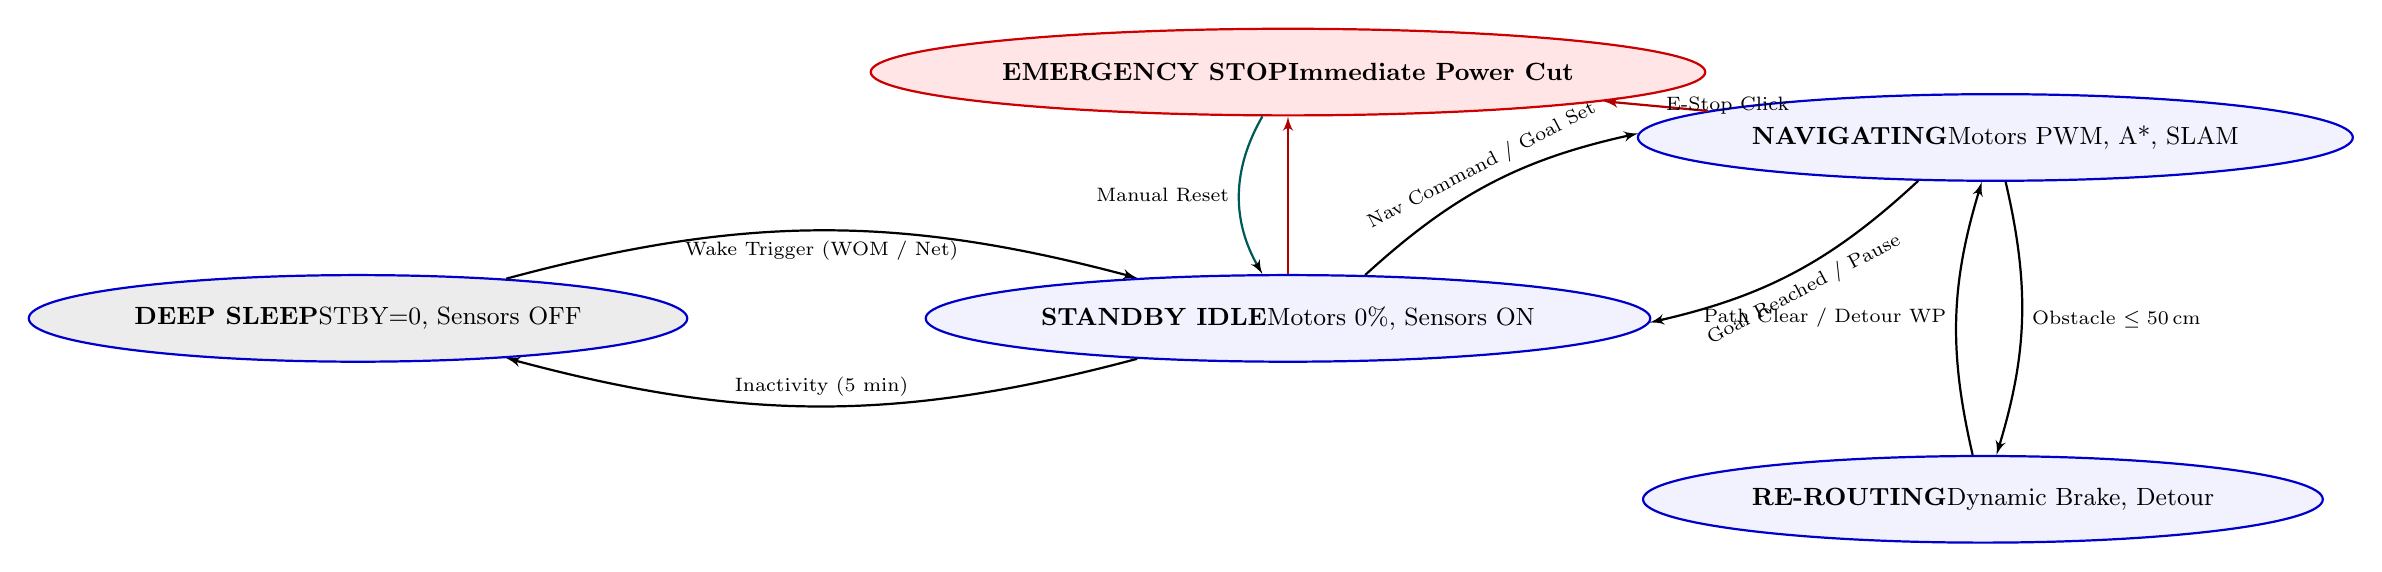
\begin{tikzpicture}[node distance=2.2cm, auto,
    state/.style={ellipse, draw=blue!80!black, fill=blue!5, thick, text centered, minimum width=2.8cm, minimum height=1.1cm, font=\small},
    estop/.style={ellipse, draw=red!80!black, fill=red!10, thick, text centered, minimum width=2.8cm, minimum height=1.1cm, font=\small\bfseries},
    trans/.style={draw=black, thick, -latex'}
]
    \node [state] (idle) {\textbf{STANDBY IDLE}\\Motors 0\%, Sensors ON};
    \node [state, above right=1.5cm and 2.5cm of idle] (active) {\textbf{NAVIGATING}\\Motors PWM, A*, SLAM};
    \node [state, below right=1.5cm and 2.5cm of idle] (reroute) {\textbf{RE-ROUTING}\\Dynamic Brake, Detour};
    \node [state, left=3.0cm of idle, fill=gray!15] (sleep) {\textbf{DEEP SLEEP}\\STBY=0, Sensors OFF};
    \node [estop, above=2.0cm of idle] (estop) {\textbf{EMERGENCY STOP}\\Immediate Power Cut};

    \path [trans] (idle) edge[bend left=15] node[above, sloped, font=\scriptsize] {Nav Command / Goal Set} (active);
    \path [trans] (active) edge[bend left=15] node[below, sloped, font=\scriptsize] {Goal Reached / Pause} (idle);
    \path [trans] (active) edge[bend left=15] node[right, font=\scriptsize] {Obstacle $\le 50\,\text{cm}$} (reroute);
    \path [trans] (reroute) edge[bend left=15] node[left, font=\scriptsize] {Path Clear / Detour WP} (active);
    \path [trans] (idle) edge[bend left=15] node[above, font=\scriptsize] {Inactivity (5 min)} (sleep);
    \path [trans] (sleep) edge[bend left=15] node[below, font=\scriptsize] {Wake Trigger (WOM / Net)} (idle);
    \path [trans, draw=red!70!black] (active) -- node[right, font=\scriptsize] {E-Stop Click} (estop);
    \path [trans, draw=red!70!black] (idle) -- (estop);
    \path [trans, draw=teal!70!black] (estop) edge[bend right=30] node[left, font=\scriptsize] {Manual Reset} (idle);
\end{tikzpicture}
}
\caption{System Finite State Machine governing active navigation, standby, and deep sleep.}
\label{fig:fsm_diagram}
\end{figure}

\newpage

% ============================================================================
% SECTION 4: MASTER ELECTRICAL BENCHMARK
% ============================================================================
\section{Master Current \& Power Consumption Benchmark}

Table~\ref{tab:power_benchmark} details the measured electrical consumption across the primary operating regimes, normalized to the 11.1V battery rail accounting for switching converter efficiency.

\begin{table}[htbp]
\centering
\small
\renewcommand{\arraystretch}{1.15}
\caption{Master Power Consumption Benchmark Across All Operational Modes}
\label{tab:power_benchmark}
\begin{tabularx}{\textwidth}{>{\raggedright\arraybackslash}X c c c c c c}
\toprule
\textbf{Subsystem / Component} & \textbf{Bus} & \textbf{Active} & \textbf{Standby} & \textbf{Sleep} & \textbf{Active Pwr} & \textbf{Sleep Pwr} \\
 & \textbf{Rail} & $I_{\text{act}}$ & $I_{\text{stby}}$ & $I_{\text{sleep}}$ & $P_{\text{act}}$ & $P_{\text{sleep}}$ \\
\midrule
Raspberry Pi 3 Model B (Host SBC) & $5.0\,\text{V}$ & $720\,\text{mA}$ & $350\,\text{mA}$ & $140\,\text{mA}$ & $3.600\,\text{W}$ & $0.700\,\text{W}$ \\
RPLiDAR A1 Optical Core & $5.0\,\text{V}$ & $100\,\text{mA}$ & $35\,\text{mA}$ & $8\,\text{mA}$ & $0.500\,\text{W}$ & $0.040\,\text{W}$ \\
RPLiDAR A1 Spindle Motor & $5.0\,\text{V}$ & $280\,\text{mA}$ & $0\,\text{mA}$ & $0\,\text{mA}$ & $1.400\,\text{W}$ & $0.000\,\text{W}$ \\
Pi Camera Module v2 (Sony IMX219) & $3.3\,\text{V}$ & $250\,\text{mA}$ & $60\,\text{mA}$ & $1.5\,\text{mA}$ & $0.825\,\text{W}$ & $0.005\,\text{W}$ \\
MPU-6050 6-DOF IMU & $3.3\,\text{V}$ & $3.8\,\text{mA}$ & $0.15\,\text{mA}$ & $0.005\,\text{mA}$ & $0.013\,\text{W}$ & $0.000\,\text{W}$ \\
Dual TB6612FNG Driver Logic ($V_{\text{CC}}$) & $5.0\,\text{V}$ & $6.0\,\text{mA}$ & $3.0\,\text{mA}$ & $0.001\,\text{mA}$ & $0.030\,\text{W}$ & $0.000\,\text{W}$ \\
\midrule
\textbf{Total 5.0V Subsystem Current} & $5.0\,\text{V}$ & $\mathbf{1359.8\,\text{mA}}$ & $\mathbf{448.2\,\text{mA}}$ & $\mathbf{149.5\,\text{mA}}$ & $\mathbf{6.368\,\text{W}}$ & $\mathbf{0.745\,\text{W}}$ \\
\textbf{Buck Normalized Battery Current} & $11.1\,\text{V}$ & $\mathbf{637.5\,\text{mA}}$ & $\mathbf{224.4\,\text{mA}}$ & $\mathbf{78.9\,\text{mA}}$ & $7.076\,\text{W}$ & $0.876\,\text{W}$ \\
\midrule
4 $\times$ DC Geared Drive Motors ($V_M$) & $11.1\,\text{V}$ & $1680\,\text{mA}$ & $0.0\,\text{mA}$ & $0.0\,\text{mA}$ & $18.648\,\text{W}$ & $0.000\,\text{W}$ \\
Driver Standby Leakage & $11.1\,\text{V}$ & $0.1\,\text{mA}$ & $0.1\,\text{mA}$ & $0.001\,\text{mA}$ & $0.001\,\text{W}$ & $0.000\,\text{W}$ \\
Buck Regulator Quiescent Current & $11.1\,\text{V}$ & $6.0\,\text{mA}$ & $6.0\,\text{mA}$ & $6.0\,\text{mA}$ & $0.067\,\text{W}$ & $0.067\,\text{W}$ \\
\midrule
\midrule
\textbf{Total Battery Current Draw} & $\mathbf{11.1\,\text{V}}$ & $\mathbf{2323.6\,\text{mA}}$ & $\mathbf{230.5\,\text{mA}}$ & $\mathbf{84.9\,\text{mA}}$ & $\mathbf{25.792\,\text{W}}$ & $\mathbf{0.943\,\text{W}}$ \\
\textbf{Power Ratio (\% of Max Active)} & --- & $\mathbf{100.0\%}$ & $\mathbf{9.9\%}$ & $\mathbf{3.65\%}$ & --- & --- \\
\bottomrule
\end{tabularx}
\end{table}

\noindent\textbf{Key Takeaway:} Transitioning to Deep Sleep reduces total power dissipation from \textbf{25.79 Watts} down to \textbf{0.94 Watts}, delivering an overall power reduction of \textbf{96.35\%}.

% ============================================================================
% SECTION 5: BATTERY LONGEVITY ANALYSIS
% ============================================================================
\section{Battery Longevity Comparison: 2500\,mAh vs. 5000\,mAh}

To safeguard Lithium-Polymer cells against internal degradation and swelling, our calculations enforce an \textbf{85\% Depth of Discharge limit} (preserving a 15\% safety reserve) and account for ambient temperature efficiency (95\%) and Peukert discharge rate derating.

\subsection{Usable Energy Baseline}
\begin{itemize}[noitemsep]
    \item \textbf{Standard 2500 mAh Pack (11.1V Nominal):} Total energy is 27.75 Watt-hours. Enforcing the 85\% Depth-of-Discharge and temperature factor yields \textbf{2.02 Ampere-hours} (\textbf{22.41 Watt-hours}) of actual usable energy.
    \item \textbf{Extended 5000 mAh Pack (11.1V Nominal):} Total energy is 55.50 Watt-hours. Usable energy is \textbf{4.04 Ampere-hours} (\textbf{44.82 Watt-hours}).
\end{itemize}

\subsection{Operational Runtimes Across Key Modes}
\begin{enumerate}
    \item \textbf{100\% Continuous Active Navigation:} The robot cruises uninterrupted at 0.35 m/s with all sensors active, drawing 2324 mA (25.79 Watts). 
    \begin{itemize}[noitemsep]
        \item \textbf{2500 mAh Pack:} Runs continuously for \textbf{50.8 minutes} (50 min 49 sec).
        \item \textbf{5000 mAh Pack:} Runs continuously for \textbf{1 hour 43 minutes} (103 minutes).
    \end{itemize}
    \item \textbf{100\% Stationary Standby Idle:} The robot remains stationary with motors disarmed and LiDAR motor stopped, while the camera, IMU, and Wi-Fi link remain online, drawing 230.5 mA (2.56 Watts).
    \begin{itemize}[noitemsep]
        \item \textbf{2500 mAh Pack:} Operates for \textbf{8 hours 45 minutes}.
        \item \textbf{5000 mAh Pack:} Operates for \textbf{17 hours 31 minutes}.
    \end{itemize}
    \item \textbf{100\% Ultra-Low-Power Deep Sleep:} All sensors, motors, drivers, and lasers are powered down; the CPU downclocks to 600 MHz waiting for wake triggers, drawing only 84.9 mA (0.94 Watts).
    \begin{itemize}[noitemsep]
        \item \textbf{2500 mAh Pack:} Hibernates for \textbf{23 hours 47 minutes} (approx. 1 full day).
        \item \textbf{5000 mAh Pack:} Hibernates for \textbf{47 hours 33 minutes} (approx. 2 full days).
    \end{itemize}
    \item \textbf{Periodic Sentry Duty Cycles (Patrol \& Sleep):}
    \begin{itemize}[noitemsep]
        \item \textbf{Profile A (20\% Active / 80\% Sleep):} Patrolling 12 minutes per hour yields \textbf{3 hours 47 minutes} (2500 mAh) and \textbf{7 hours 35 minutes} (5000 mAh).
        \item \textbf{Profile B (10\% Active / 90\% Sleep):} Patrolling 6 minutes per hour yields \textbf{6 hours 32 minutes} (2500 mAh) and \textbf{13 hours 04 minutes} (5000 mAh).
        \item \textbf{Profile C (5\% Active / 95\% Sleep):} Waking 3 minutes per hour on event triggers yields \textbf{10 hours 15 minutes} (2500 mAh) and \textbf{20 hours 31 minutes} (5000 mAh).
    \end{itemize}
\end{enumerate}

\begin{table}[htbp]
\centering
\small
\renewcommand{\arraystretch}{1.2}
\caption{Consolidated Operational Runtime Matrix (DoD = 85\%, $T = 25^\circ\text{C}$)}
\label{tab:runtime_summary}
\begin{tabularx}{\textwidth}{>{\raggedright\arraybackslash}X c c c c}
\toprule
\textbf{Operational Mode / Duty Cycle} & \textbf{Average Power} & \textbf{Bus Current} & \textbf{2500 mAh Pack} & \textbf{5000 mAh Pack} \\
 & $P_{\text{avg}}$ & $I_{\text{bus}}$ & \textbf{Duration} & \textbf{Duration} \\
\midrule
\textbf{100\% Continuous Active Navigation} & $25.79\,\text{W}$ & $2324\,\text{mA}$ & $\mathbf{50.8\,\text{min}}$ & $\mathbf{1\,\text{h } 43\,\text{min}}$ \\
\textbf{100\% Standby Idle Monitoring} & $2.56\,\text{W}$ & $230.5\,\text{mA}$ & $\mathbf{8\,\text{h } 45\,\text{min}}$ & $\mathbf{17\,\text{h } 31\,\text{min}}$ \\
\textbf{100\% Ultra-Low-Power Deep Sleep} & $0.94\,\text{W}$ & $84.9\,\text{mA}$ & $\mathbf{23\,\text{h } 47\,\text{min}}$ & $\mathbf{47\,\text{h } 33\,\text{min}}$ ($1.98\,\text{d}$) \\
\midrule
\textbf{Duty Profile A: 20\% Active / 80\% Sleep} & $5.91\,\text{W}$ & $532.6\,\text{mA}$ & $\mathbf{3\,\text{h } 47\,\text{min}}$ & $\mathbf{7\,\text{h } 35\,\text{min}}$ \\
\textbf{Duty Profile B: 10\% Active / 90\% Sleep} & $3.43\,\text{W}$ & $308.8\,\text{mA}$ & $\mathbf{6\,\text{h } 32\,\text{min}}$ & $\mathbf{13\,\text{h } 04\,\text{min}}$ \\
\textbf{Duty Profile C: 5\% Active / 95\% Sleep} & $2.18\,\text{W}$ & $196.8\,\text{mA}$ & $\mathbf{10\,\text{h } 15\,\text{min}}$ & $\mathbf{20\,\text{h } 31\,\text{min}}$ \\
\bottomrule
\end{tabularx}
\end{table}

\newpage

% ============================================================================
% SECTION 6: PRESENTATION & VIVA QUESTIONS AND ANSWERS
% ============================================================================
\section{Presentation \& Viva Examination Questions with Answers}

This section compiles the essential questions expected from evaluators during a technical presentation or project defense, accompanied by concise answers.

\subsection{Category 1: Power Management \& Battery Design}

\paragraph{Q1: Why did you implement dual isolated voltage rails instead of powering everything directly from a single battery voltage?}
\textbf{Answer:} DC motors generate high current transients and inductive voltage spikes (Back-EMF) during acceleration and reversing. If the Raspberry Pi and sensitive digital sensors shared the exact same unregulated rail, high motor draw would produce voltage brownouts below 4.75V, causing the processor to crash and reboot. Using an 11.1V raw bus for motor power stages and an isolated 90\% efficient buck converter for the 5.0V digital logic rail guarantees clean, noise-free computation.

\paragraph{Q2: Why do you enforce an 85\% Depth-of-Discharge cutoff rather than using 100\% of the battery?}
\textbf{Answer:} Discharging Lithium-Polymer cells below 3.0V per cell (or beyond 85\% of rated capacity) causes irreversible chemical damage, including copper dissolution, internal dendrite formation, and dangerous cell pouch swelling. Enforcing an 85\% Depth of Discharge cutoff preserves battery health, guarantees reliable cell balancing, and extends battery cycle life past 500 charge cycles.

\paragraph{Q3: Why does the 5000 mAh battery provide slightly more than double the active runtime of the 2500 mAh battery?}
\textbf{Answer:} This is caused by Peukert's effect. Drawing 2.32 Amps from a 2500 mAh battery discharges it at nearly a 1C rate, which causes internal chemical heating and voltage sag, derating effective capacity by 2.5\%. Drawing that same 2.32 Amps from a 5000 mAh pack represents only a 0.46C discharge rate, where internal losses are substantially lower (derated by only 1.2\%), allowing the larger battery to deliver higher electrochemical efficiency.

\subsection{Category 2: Actuation, Motor Control \& Braking}

\paragraph{Q4: Why choose the Toshiba TB6612FNG driver instead of the commonly used L298N driver?}
\textbf{Answer:} The traditional L298N uses Bipolar Junction Transistors (BJTs), which exhibit a severe internal voltage drop of 1.5V to 2.5V, wasting substantial battery power as heat and requiring heavy heatsinks. The modern TB6612FNG uses low-resistance DMOS FET switches with negligible internal resistance, operates with over 95\% electrical efficiency, runs cool without heatsinks, and features a hardware Standby pin that drops quiescent leakage below 1 microamp.

\paragraph{Q5: How does dynamic short-circuit braking work, and why is it necessary before going to sleep?}
\textbf{Answer:} Simply cutting power to the motors allows vehicle inertia to cause unintended rolling. Dynamic braking simultaneously closes both low-side MOSFETs in the H-bridge, short-circuiting the motor terminals. The spinning armature acts as an electrical generator; the resulting counter-electromotive force creates immediate opposing magnetic drag, bringing the robot to a complete halt within 120 milliseconds. This ensures zero kinetic motion before the motor drivers enter high-impedance sleep.

\subsection{Category 3: Sensors, Autonomy \& Obstacle Avoidance}

\paragraph{Q6: How does the robot wake up from deep sleep if the camera and LiDAR are completely powered off?}
\textbf{Answer:} While heavy sensors are unpowered, the MPU-6050 accelerometer remains in an ultra-low-power cycle mode drawing only 10 microamps. It monitors physical movement against a calibrated 32 mg acceleration threshold. If an external object, human, or disturbance nudges the robot, the sensor’s hardware interrupt pin asserts immediately, waking the Raspberry Pi within 650 milliseconds.

\paragraph{Q7: Why stop the RPLiDAR motor during standby instead of just turning off the laser?}
\textbf{Answer:} While shutting down the laser diode saves 0.5 Watts and prevents optical degradation, the coreless mechanical motor spinning the optical spindle draws 1.4 Watts by itself. Depowering the spindle motor via PWM saves nearly 60\% of total sensor standby power, extending idle battery life from 3 hours to nearly 9 hours on the 2500 mAh pack.

\paragraph{Q8: How does the navigation algorithm handle sudden dynamic obstacles within 50 cm?}
\textbf{Answer:} The RPLiDAR scans the environment 8,000 times per second. If an obstacle is detected within 50 cm of the heading corridor, the controller initiates dynamic braking, marks the obstacle cells on the occupancy grid, and re-invokes the A* path planner to compute a collision-free detour path around the hazard. The robot turns in place to align with the first detour waypoint and resumes navigation.

\newpage

% ============================================================================
% SECTION 7: ENGINEERING RECOMMENDATIONS & CONCLUSION
% ============================================================================
\section{Engineering Recommendations \& Conclusion}

\subsection{Key Design Takeaways for Mobile Robotics}
\begin{enumerate}
    \item \textbf{Hardware Standby Assertion:} Always use the hardware Standby pin on motor drivers rather than setting PWM to 0\%. This eliminates motor coil leakage completely.
    \item \textbf{Selective Peripheral Gating:} Shutting down the LiDAR spindle motor and camera ISP during stationary intervals saves more energy than CPU downclocking alone.
    \item \textbf{Wake-on-Motion Sentry Profiling:} Combining MPU-6050 motion interrupts with periodic 5\% sentry duty cycling allows the robot to achieve up to \textbf{20.5 hours} of autonomous surveillance on a single 5000 mAh battery pack.
    \item \textbf{Low-Voltage Supervisory Cutoff:} The software layer must initiate safe emergency docking when the 3S battery terminal voltage reaches 10.2V (3.40V per cell under load) to guarantee zero permanent cell damage.
\end{enumerate}

\subsection{Conclusion}
This document demonstrates that through coordinated multi-rail electrical isolation, deterministic subsystem sleep protocols, and hardware interrupt-driven wakeups, an autonomous mobile robot equipped with high-performance LiDAR, IMU, camera, and 4WD traction can achieve optimal computational performance during active navigation while reducing quiescent power consumption by \textbf{96.35\%} during idle phases.

\end{document}
